For CSS-hovedenheden er der udviklet en række diagrammer ud fra applikationsmodel-metoden. De bygger videre på domænemodellen for hele systemet.
Der er et sekvensdiagram på figur \ref{fig:CSS_hovedenhed_SD} for alle de aktuelle use-cases som beskriver systemets virkemåde.
Ud fra dette er der lavet et klassediagram på figur \ref{fig:CSS_hovedenhed_Class} som dækker de forskellige use-cases med controller klasser og kommunikationen til PC via RS232 og X10-udtag via X10.


\begin{figure}[!htb]
	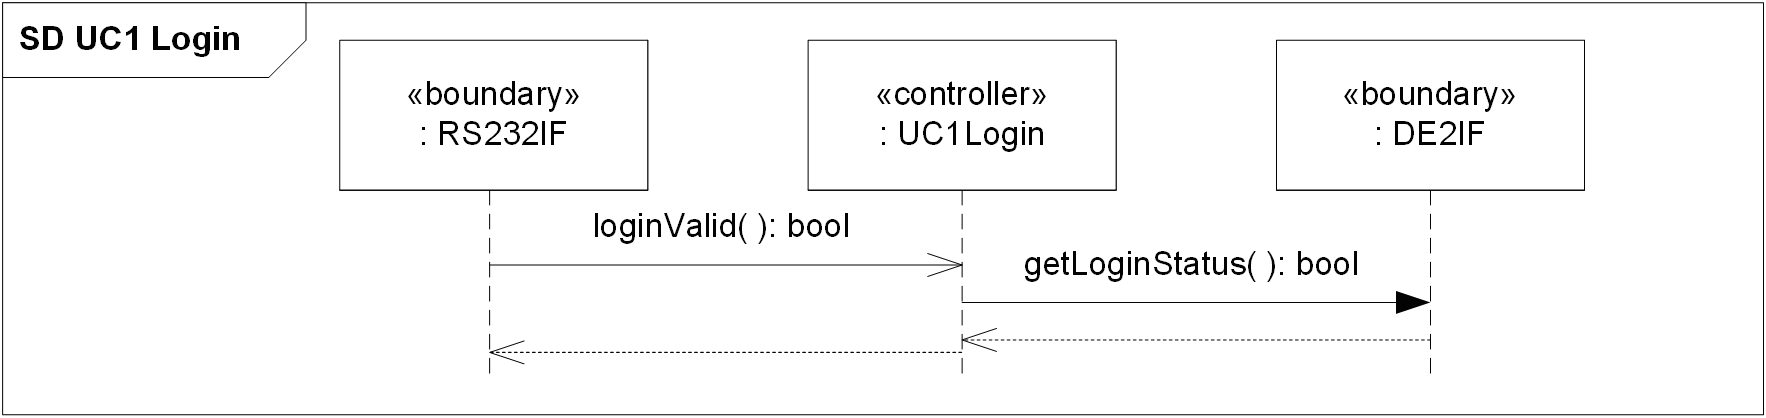
\includegraphics[width=\textwidth]{billeder/uml/CSS_hovedenhed_SD}
     \caption{Use-case sekvensdiagrammer for CSS-hovedenhed}
     \label{fig:CSS_hovedenhed_SD}
\end{figure}

\begin{figure}[!htb] \centering
     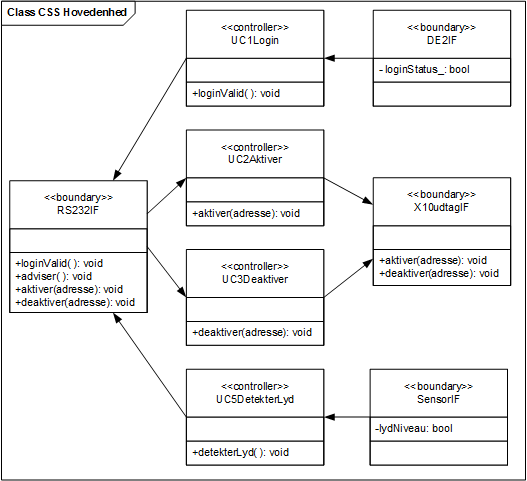
\includegraphics[width=0.8\textwidth]{billeder/uml/CSS_hovedenhed_Class}
     \caption{Klassediagram for CSS-hovedenhed}
     \label{fig:CSS_hovedenhed_Class}
\end{figure}

Under designfasen og implementeringen laves der en række støtte metoder til klasserne. Det endelige klassediagram kan ses på  figur \ref{fig:CSS_hovedenhed_Class_Static}. De globale funktionaliteter som egentlig strider mod objekt-orienteret programmering er resultatet af, at arbejde med software til en microcontroller som har en række autonomo funktionaliteter som bliver eksekveret fra udefra-kommende hardware signaler.

\begin{figure}[!htb] \centering
     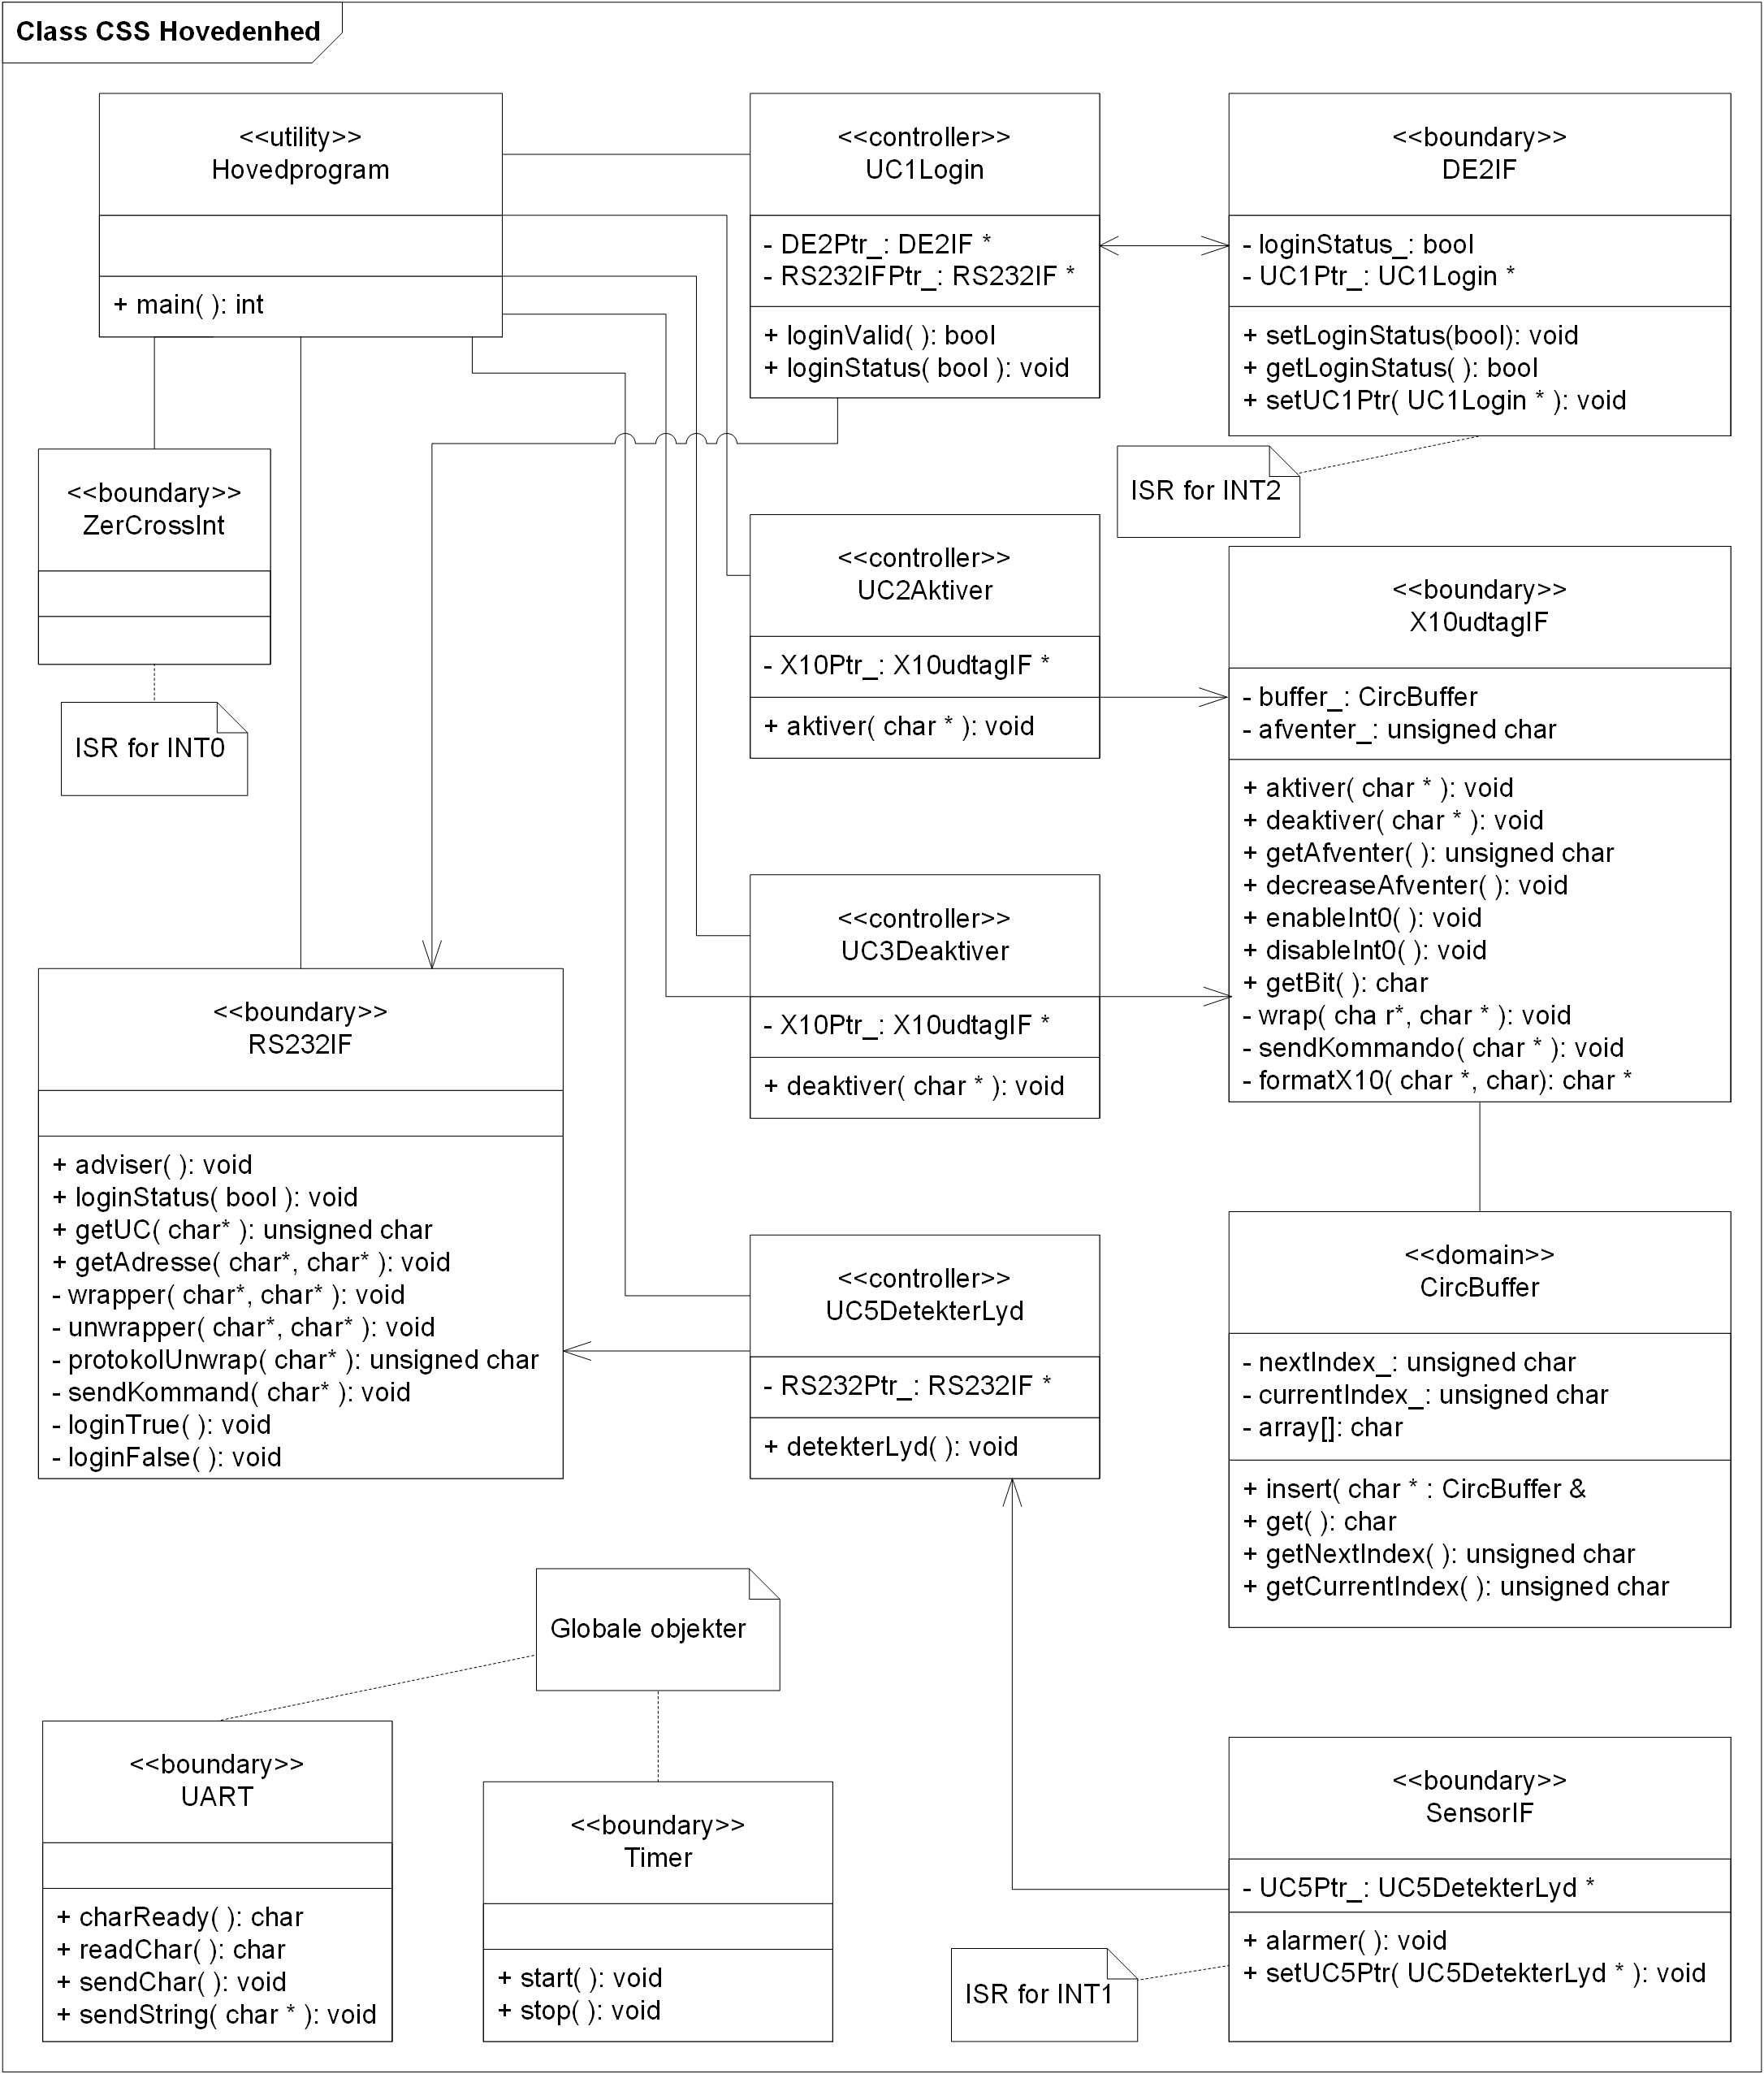
\includegraphics[width=\textwidth]{billeder/uml/CSS_hovedenhed_Class_Static}
     \caption{Statisk klassediagram for CSS-hovedenhed}
     \label{fig:CSS_hovedenhed_Class_Static}
\end{figure}